\newpage
\section{Programming exercise : Applying decision trees and k-nearest neighbors \problemworth{55}}

\section*{Introduction}

\begin{figure}[ht]
\centering
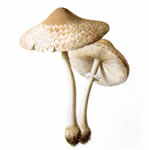
\includegraphics[scale=2.5]{mushroom.jpg}
\end{figure}

In this problem, we will work on a mushroom classification task. The dataset is adapted from the \href{https://archive.ics.uci.edu/ml/datasets/mushroom}{UCI Machine Learning Repository} and it contains descriptions of hypothetical samples corresponding to 23 species of gilled mushrooms. Each mushroom is described in terms of physical characteristics, and the goal is to classify mushrooms as \emph{edible} or \emph{poisonous}. We will apply decision trees and k-nearest neighbors. Since this dataset is relatively simple for classification, we only use 6 features out of 22 features in the original dataset. Features we use include: 
cap-shape, cap-color, gill-color, stalk-root, veil-type, ring-number.


For all the coding, please refer to the following Colab notebook  
\href{https://colab.research.google.com/drive/13_JuaV8-uwTBO7YEheYGm3cjl8DZB8HA?usp=sharing}{Fall2022-CM146-HW1.ipynb}. 

\textbf{Before executing or writing down any code, please make a copy of the notebook and save it to your own google drive by clicking the “File” $\rightarrow$ “Save a copy in Drive”.} 

\begin{figure}[ht]
\centering
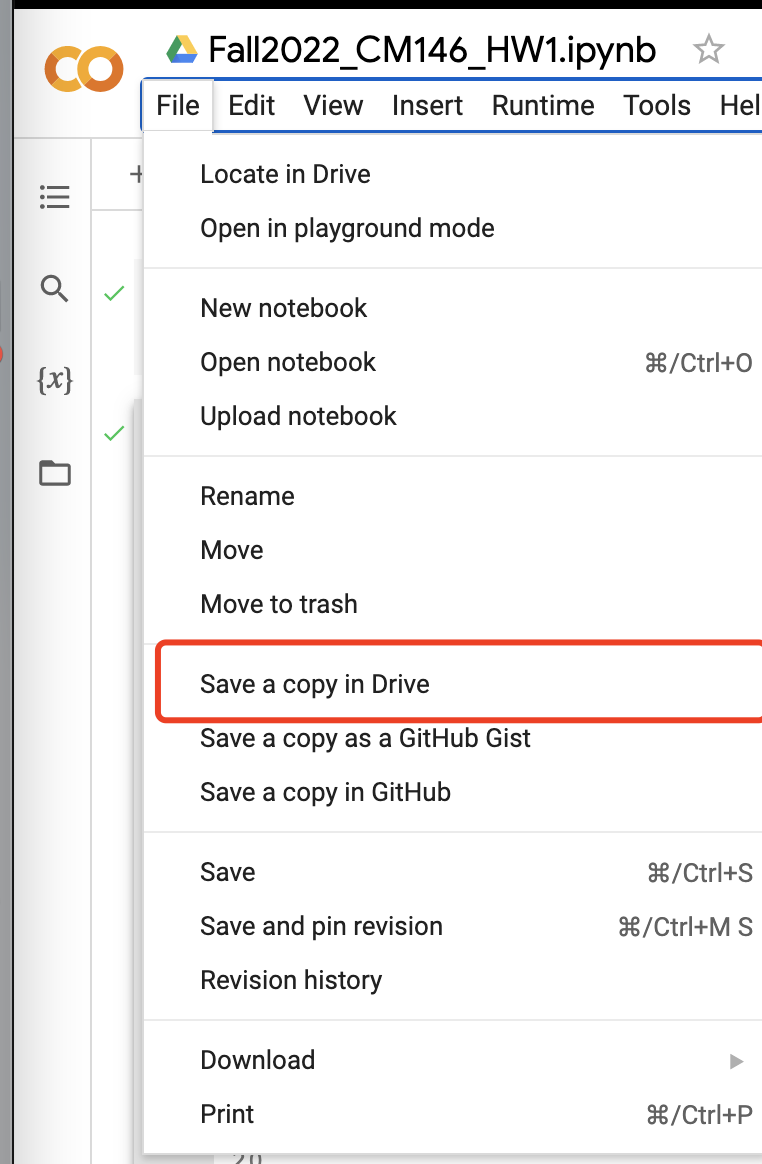
\includegraphics[scale=0.25]{save-colab-to-drive.png}
\end{figure}

You will probably be prompted to log into your Google account. Please make sure all the work you implement is done on your own saved copy. You won’t to able to make changes on the the original notebook shared with the entire class.

The notebook has marked blocks where you need to code:
\begin{verbatim}
### ========== TODO : START ========== ###
### ========== TODO : END ========== ###
\end{verbatim}

\section*{Submission instructions for programming problems}
\begin{itemize}
\item Please save the execution output in your notebook. When submitting, please export the notebook to a \verb|.ipynb| file by clicking ``File'' $\rightarrow$ ``Download .ipynb'' and upload the notebook to BruinLearn.

\item
Your code should be commented appropriately. Importantly:
\begin{itemize}[nosep]
\item Your name should be at the top of the file.
\item Each class and method should have an appropriate doctsring.
\item Include some comments for anything complicated.
\end{itemize}

There are many possible solutions to this assignment, which makes coding style and comments important for graders to conveniently understand the code. 

\item Please submit all the plots and the rest of the solutions (other than codes) to Gradescope.
\end{itemize}


\subsection{Visualizing Features \problemworth{5}}
One of the first things to do before trying any formal machine learning technique is to dive into the data. This can include looking for funny values in the data, looking for outliers, looking at the range of feature values, what features seem important, etc.
We have already included the code for loading the data, converting all the categorical features to numerical one.

Make histograms for each feature, separating the examples by class (i.e., edible or poisonous).
This should produce 6 plots, one for each feature, and each plot should have two overlapping histograms, with the color of the histogram indicating the class. 
The code has been included in \texttt{plot\_histograms} and \texttt{plot\_histogram} functions, and you do not need to code by yourself.

For each feature, what trends do you observe in the data? (Please only describe the general trend. No need for more than two sentences per feature.) 

\subsection{Training and Evaluating Models \problemworth{55}}

Now, let's use \verb|scikit-learn| to train a \verb|DecisionTreeClassifier| and \verb|KNeighborsClassifier| on the data.
Using the predictive capabilities of the \verb|scikit-learn| package can be carried out in three steps: initializing the model, fitting it to the training data, and predicting new values.

\begin{enumerate}

\item \itemworth{5} Before trying out any classifier, it is often useful to establish a \emph{baseline}. We have implemented one simple baseline classifier, \verb|MajorityVoteClassifier|, that always predicts the majority class from the training set. Read through the \verb|MajorityVoteClassifier| and its usage and make sure you understand how it works.

Your goal is to implement and evaluate another baseline classifier, \verb|RandomClassifier|, that predicts a target class according to the distribution of classes in the training data set. For example, if 85\% of the examples in the training set have \verb|edible = 0| and 15\% have \verb|edible = 1|, then, when applied to a test set, \verb|RandomClassifier| should randomly predict 85\% of the examples as \verb|edible = 0| and 15\% as \verb|edible = 1|.

Implement the missing portions of \verb|RandomClassifier| according to the provided specifications. Then train your \verb|RandomClassifier| on the entire training data set, and evaluate its training error. 


\item \itemworth{5} Now that we have a baseline, train and evaluate a \verb|DecisionTreeClassifier| (using the class from \verb|scikit-learn| and referring to the documentation as needed). Make sure you initialize your classifier with the appropriate parameters; in particular, use the `entropy' criterion discussed in class. What is the training error of this classifier?




\item \itemworth{10} Similar to the previous question, train and evaluate a \verb|KNeighborsClassifier| (using the class from \verb|scikit-learn| and referring to the documentation as needed). Use $k$=3, 11 and 19 as the number of neighbors and report the training error of this classifier. If we implement KNN model from scratch, what operations we should do in the \verb|fit| method?


\item \itemworth{10} So far, we have looked only at training error, but as we learned in class, training error is a poor metric for evaluating classifiers. Let's use cross-validation instead.

Implement the missing portions of \verb|error(...)| according to the provided specifications. You may find it helpful to use \verb|StratifiedShuffleSplit(...)| from \verb|scikit-learn|. To ensure that we always get the same splits across different runs (and thus can compare the classifier results), set the \verb|random_state| parameter to be the same (e.g., 0).


Next, use your \verb|error(...)| function to evaluate the training error and (cross-validation) test error and test micro averaged \href{https://scikit-learn.org/stable/modules/generated/sklearn.metrics.f1_score.html?highlight=f1\%20score#sklearn.metrics.f1_score}{F1 Score} of each of your four models (for the \verb|KNeighborsClassifier|, use $k=11$). To do this, generate a random $85/15$ split of the training data, train each model on the $85\%$ fraction, evaluate the error on both the $85\%$ and the $15\%$ fraction, and repeat this $100$ times to get an average result.


\item \itemworth{10} One way to find out the best value of $k$ for \verb|KNeighborsClassifier| is $n$-fold cross validation.
Find out the best value of $k$ using 5-fold cross validation and the F1 Score metric. Run cross validation for all odd numbers ranging from 1 to 100 as the number of neighbors.

Then plot the validation score against the number of neighbors, $k$. Include this plot in your writeup. What is the best value of $k$ and what is the corresponding score?

You may find the \verb|cross_val_score(...)| from \verb|scikit-learn| helpful. 


\item \itemworth{10} One problem with decision trees is that they can \emph{overfit} to training data, yielding complex classifiers that do not generalize well to new data. Let's see whether this is the case.

One way to prevent decision trees from overfitting is to limit their depth. Run 20-fold cross-validation for increasing depth limits $1,2,\ldots,20$. 

Then plot the average training F1 Score and test F1 score against the depth limit. Include this plot in your writeup, making sure to label all axes and include a legend for your classifiers. What is the best depth limit to use for this data? Do you see overfitting? Justify your answers using the plot.

You may find \verb|cross_validate| from \verb|scikit-learn| helpful when you want both training scores and validation scores.

\end{enumerate}
